% Module C - Economic Feasibility Assessment
% Compiles with XeLaTeX (Overleaf: Menu -> Compiler -> XeLaTeX) or `tectonic main.tex`.
% Every number and chart in this document is produced by econ_model.py (see evidence_numbers.txt).
\documentclass[10pt,a4paper]{article}

\usepackage{fontspec}
\IfFontExistsTF{Times New Roman}{\setmainfont{Times New Roman}}{\setmainfont{TeX Gyre Termes}}
\usepackage[a4paper,margin=2cm,top=2cm,bottom=2.2cm]{geometry}
\usepackage{graphicx}
\usepackage{array,tabularx,longtable,multirow}
\usepackage[table]{xcolor}
\usepackage{amsmath}
\usepackage{pifont}
\usepackage{enumitem}
\usepackage{float}
\usepackage{needspace}
\usepackage{caption}
\usepackage{titlesec}
\usepackage{tikz}
\usetikzlibrary{positioning,arrows.meta,calc,shapes.symbols}
\usepackage[most]{tcolorbox}
\usepackage{xurl}
\usepackage[hidelinks]{hyperref}
\hypersetup{pdftitle={Autonomous UAV System for Forest Fire Monitoring - Module C Economic Feasibility Assessment}}

\setlength{\parindent}{0pt}
\setlength{\parskip}{4pt}
\renewcommand{\arraystretch}{1.18}
\captionsetup{font=small,labelfont=bf,labelsep=colon}
\setlist{itemsep=1pt,topsep=3pt}
\titleformat{\section}{\Large\bfseries}{\thesection}{0.6em}{}
\titleformat{\subsection}{\large\bfseries}{\thesubsection}{0.6em}{}
\titlespacing*{\section}{0pt}{10pt}{6pt}
\titlespacing*{\subsection}{0pt}{8pt}{4pt}
\newcolumntype{L}[1]{>{\raggedright\arraybackslash}p{#1}}
\newcolumntype{R}[1]{>{\raggedleft\arraybackslash}p{#1}}
\newcolumntype{Y}{>{\raggedright\arraybackslash}X}

\definecolor{passgreen}{HTML}{1E7B34}
\definecolor{warnamber}{HTML}{A65F00}
\definecolor{failred}{HTML}{B3261E}
\definecolor{headgray}{HTML}{F2F2F2}
\definecolor{vizblue}{HTML}{2A78D6}
\definecolor{vizorange}{HTML}{EB6834}
\newcommand{\PASS}{\textcolor{passgreen}{\textbf{\ding{51}\,MET}}}
\newcommand{\head}[1]{\textbf{#1}}
\newcommand{\file}[1]{\texttt{\small #1}}
\newcommand{\src}[1]{\textcolor{passgreen}{\textbf{[S]}}\,#1}   % sourced price
\newcommand{\est}[1]{\textcolor{warnamber}{\textbf{[E]}}\,#1}   % planning estimate
\newcommand{\rub}{\,RUB}

\tikzset{box/.style={draw,rounded corners=3pt,align=center,font=\small,minimum height=9mm,inner sep=4pt},
         arr/.style={-{Stealth[length=2.2mm]},thick}}

% key-number tile: value, label, note
\newcommand{\kpi}[3]{\begin{tikzpicture}\node[draw=gray!35,fill=headgray,rounded corners=3pt,minimum width=2.7cm,
  minimum height=1.75cm,align=center,inner sep=3pt]{{\LARGE\bfseries #1}\\[2pt]{\small\bfseries #2}\\{\scriptsize\color{gray!70!black}#3}};\end{tikzpicture}}
% one-line takeaway box
\newtcolorbox{takeaway}{colback=vizblue!5,colframe=vizblue!70!black,boxrule=0.6pt,arc=2pt,left=6pt,right=6pt,top=3pt,bottom=3pt}
\newtcolorbox{caution}{colback=vizorange!6,colframe=vizorange!80!black,boxrule=0.6pt,arc=2pt,left=6pt,right=6pt,top=3pt,bottom=3pt}

\begin{document}

% ------------------------------------------------------------------ cover
\begin{titlepage}
\centering
{\large\bfseries BRICS HIGHSKILLS 2026\par}
\vspace{2pt}
{\bfseries AERIAL ROBOTICS COMPETITION\par}
\vspace{2pt}
{Economic Feasibility Assessment\par}
\vspace{10pt}
\rule{\textwidth}{0.6pt}
\vspace{18pt}

\raggedright
{\large\bfseries CASE 1\par}
\vspace{8pt}
{\fontsize{22}{26}\selectfont\bfseries AUTONOMOUS UAV SYSTEM\\FOR FOREST FIRE MONITORING\par}
\vspace{8pt}
{\large Economic model, cost--benefit calculation,\\comparison of technical options and recommendations\par}
\vspace{18pt}

\centering
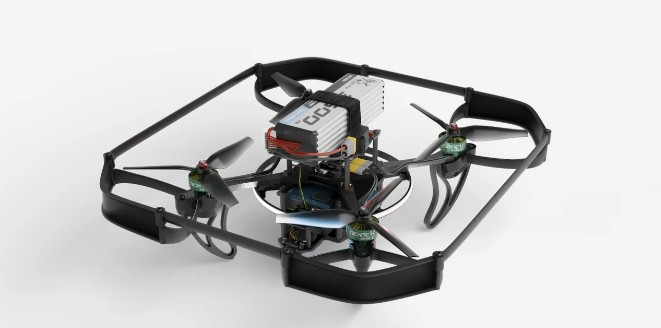
\includegraphics[width=0.62\textwidth]{figures/drone_cover.png}\par
\vspace{4pt}
{\small\textbf{Figure 1:} SKYRIS TECHNIC 6S with the team's onboard software --- the system being assessed\par}
\vspace{22pt}

{\Large\bfseries TEAM ENTITY\par}
{\Large\bfseries Workstation Number: 5\par}
\vspace{16pt}

\begin{tabularx}{\textwidth}{|L{3.2cm}|Y|}
\hline
\head{Competition} & BRICS HIGHSKILLS 2026 --- Aerial Robotics \\ \hline
\head{Case Study} & Autonomous UAV System for Forest Fire Monitoring \\ \hline
\multirow{2}{*}{\head{Team Members}} & Kamalesh Vadivelu Syamala \\
 & Bejin Paul Josephin Paul Benjamin \\ \hline
\head{Document} & Module C --- Economic Feasibility Assessment \\ \hline
\head{Assessment basis} & One forest district, 5 years, nominal RUB, prices of November 2026 \\ \hline
\head{Revision} & November 2026 \\ \hline
\end{tabularx}
\end{titlepage}
\setcounter{figure}{1}

% ------------------------------------------------------------------ at a glance
\section*{Executive Summary}
\vspace{-6pt}\rule{\textwidth}{0.4pt}

\noindent\kpi{6.21\,M}{NPV}{RUB at 18\,\%}\hfill
\kpi{74.1\,\%}{IRR}{hurdle 18\,\%}\hfill
\kpi{1.48\,yr}{Payback}{discounted 1.77\,yr}\hfill
\kpi{362\,\%}{ROI}{over 5 years}\hfill
\kpi{$-$12.5\,\%}{vs COTS drone}{same work, 5 yr}\hfill
\kpi{0.52}{fires / yr}{to break even}

\vspace{4pt}
\begin{takeaway}
\textbf{Verdict: economically feasible.} One district, two UAVs, 5 years. CAPEX 3.50\,M\rub, OPEX 1.40\,M\rub/yr,
benefits 5.20\,M\rub/yr. The investment returns in under 1.5 years and is 12.5\,\% cheaper than buying commercial thermal
drones for the same work.
\end{takeaway}

\begin{figure}[H]
\centering
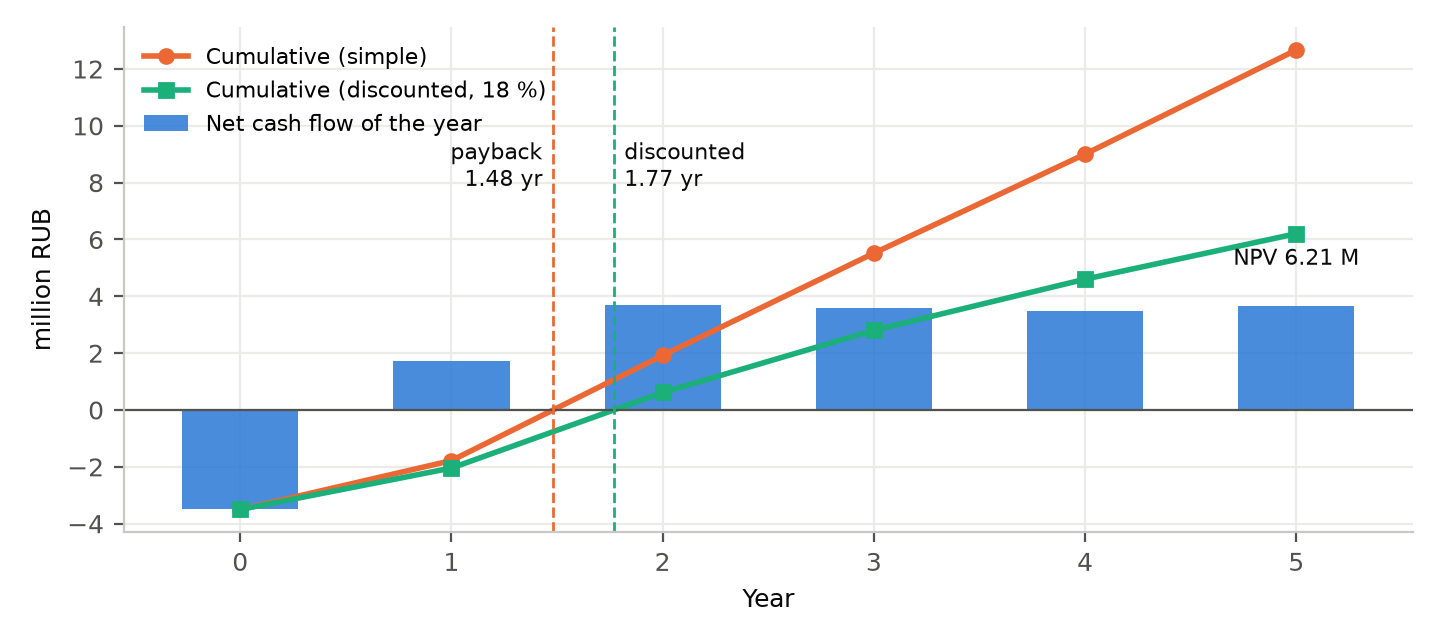
\includegraphics[width=0.9\textwidth]{figures/fig_cashflow.png}
\caption{Five-year cash flow. Cumulative cash turns positive at 1.48 years (simple) and 1.77 years (discounted).}
\end{figure}

\begin{tabularx}{\textwidth}{@{}Y Y Y@{}}
\textbf{Software, not hardware.} All parts are stock. The team's product is the onboard software, so it ships as
an update and installs on PX4 drones. &
\textbf{Proven in Module B.} 15/15 autonomous missions, campfire found in every flight, mAP@0.5 = 0.993, no crash in
61 starts. &
\textbf{Condition.} Cash savings alone do not repay the investment in 5 years; the result depends on fires caught early
(Section~9). \\
\end{tabularx}

\vspace{4pt}
{\small Base-case inputs: team model \file{economics/case1\_fire.yaml} (also on the dashboard Economics page). All numbers and
charts: \file{econ\_model.py}. Prices marked \src{} are sourced; \est{} are planning estimates.}

\newpage
% ------------------------------------------------------------------ 1
\section{Project Economic Model}

\subsection{Customer and value chain}
\textbf{Customer:} regional forestry service. \textbf{Problem:} suspected ignition points are checked by paid patrol flights or
ground crews; small fires are found late. \textbf{Our role:} the UAV flies the route, detects flame on board and sends
coordinates, before the fire grows.

\begin{figure}[H]
\centering
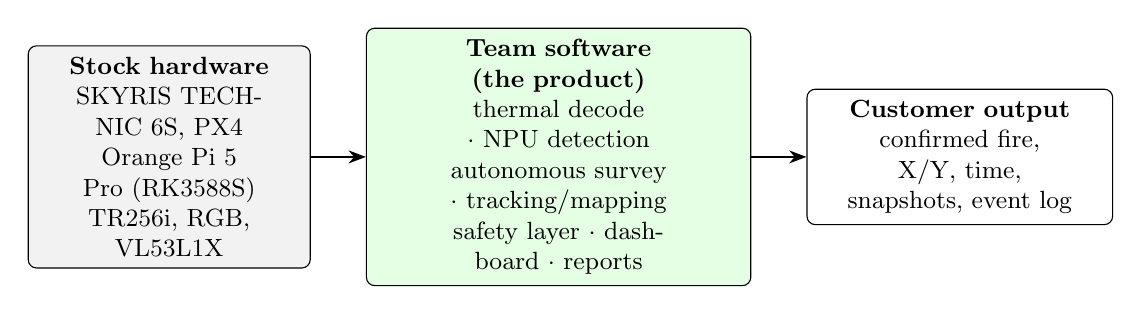
\begin{tikzpicture}[node distance=5mm and 7mm]
\node[box,fill=headgray,text width=3.3cm] (hw) {\textbf{Stock hardware}\\SKYRIS TECHNIC 6S, PX4\\Orange Pi 5 Pro (RK3588S)\\TR256i, RGB, VL53L1X};
\node[box,fill=green!10,text width=4.6cm,right=of hw] (sw) {\textbf{Team software (the product)}\\thermal decode $\cdot$ NPU detection\\autonomous survey $\cdot$ tracking/mapping\\safety layer $\cdot$ dashboard $\cdot$ reports};
\node[box,text width=3.6cm,right=of sw] (out) {\textbf{Customer output}\\confirmed fire, X/Y, time,\\snapshots, event log};
\draw[arr] (hw)--(sw); \draw[arr] (sw)--(out);
\end{tikzpicture}
\caption{Only the green block was developed by the team; everything else is bought off the shelf.}
\end{figure}

\begin{takeaway}
\textbf{Why software-only matters economically:} payload kit $\approx$ 50\,000\rub\ per UAV (no hardware R\&D) $\cdot$ all 10
Module~B defects fixed in software within the test window $\cdot$ software (1.2\,M\rub) is paid once and reused in every district.
\end{takeaway}

\subsection{Costs and benefits}
\begin{figure}[H]
\centering
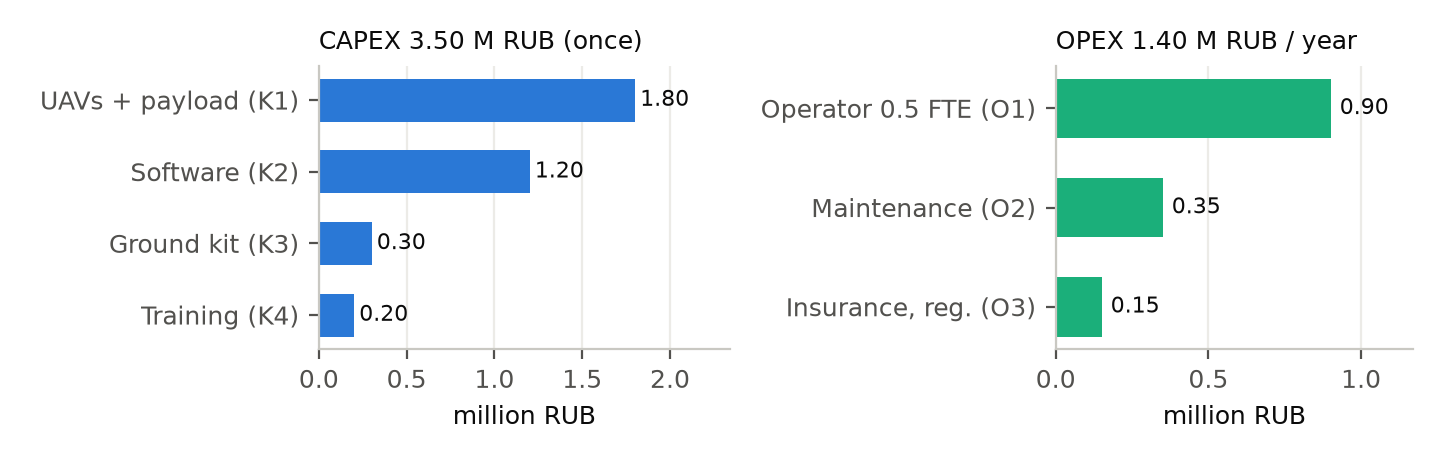
\includegraphics[width=0.92\textwidth]{figures/fig_capex_opex.png}
\caption{Where the money goes. The largest running cost is staff time, which autonomy keeps at 0.5 FTE for two UAVs.}
\end{figure}

\begin{figure}[H]
\centering
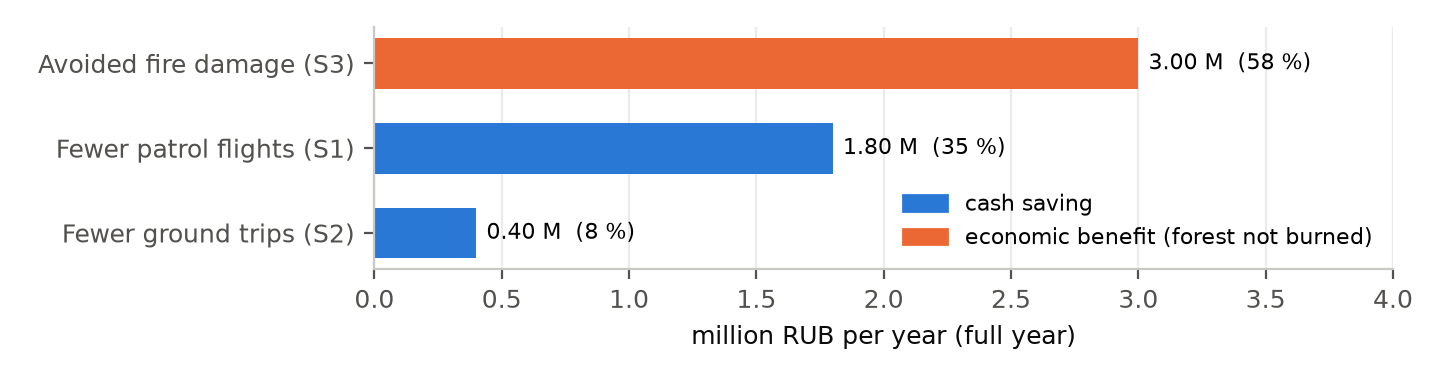
\includegraphics[width=0.92\textwidth]{figures/fig_benefits.png}
\caption{Annual benefits: 2.20\,M\rub\ cash savings and 3.00\,M\rub\ forest not burned. Non-monetary effects are in Section~10.}
\end{figure}

% ------------------------------------------------------------------ 2
\section{What the Investment Buys: Verified Prototype}

\begin{figure}[H]
\centering
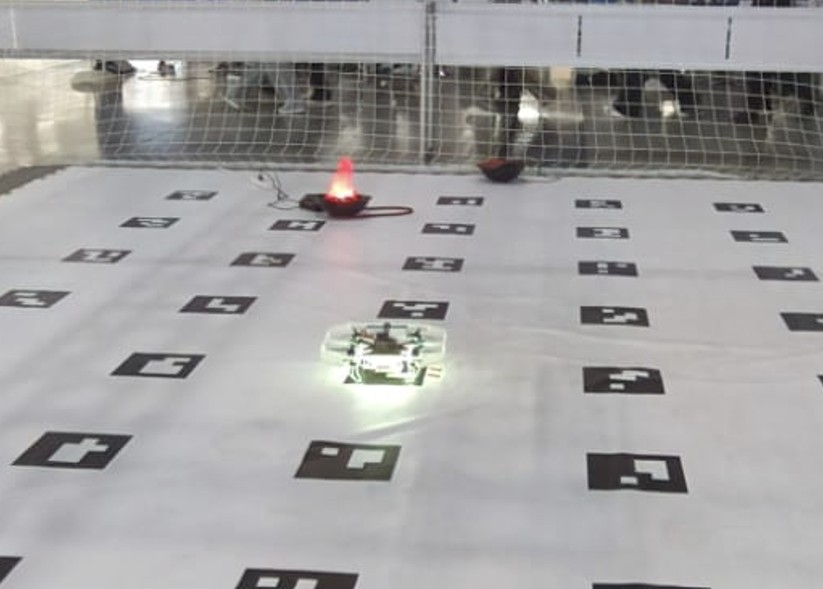
\includegraphics[height=3.3cm]{figures/photo_hover.png}\hfill
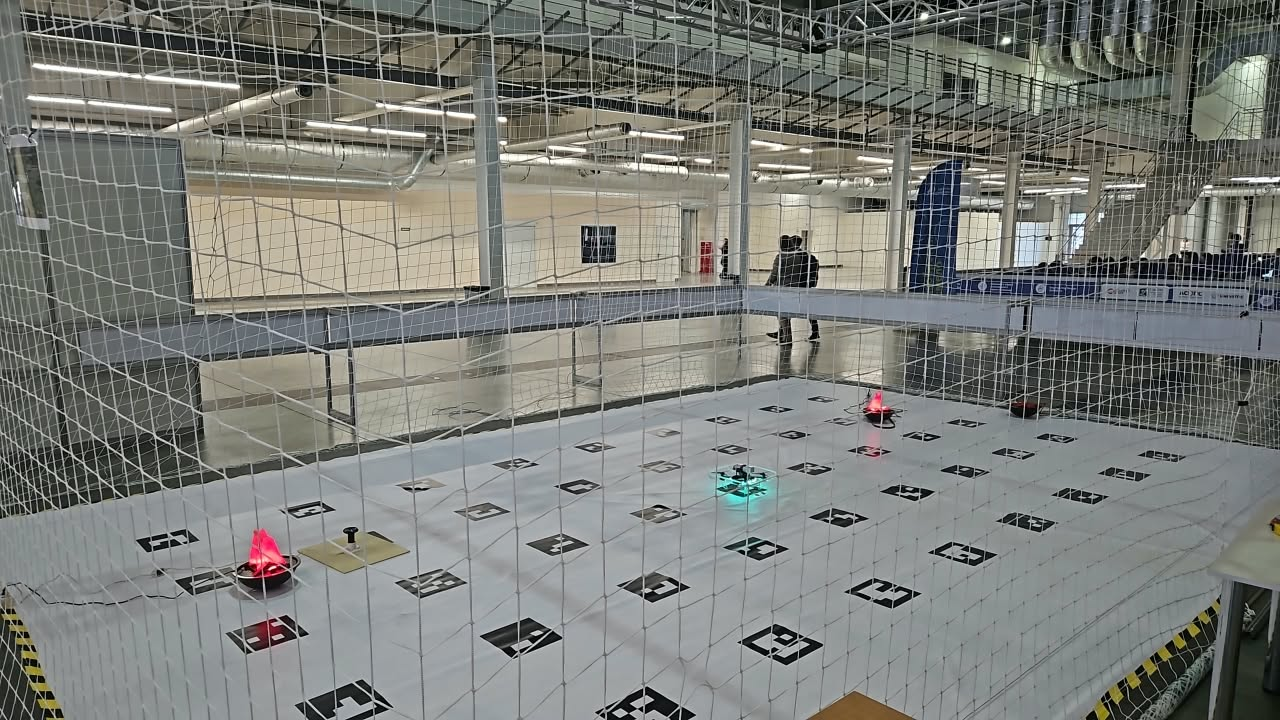
\includegraphics[height=3.3cm]{figures/photo_area.png}\hfill
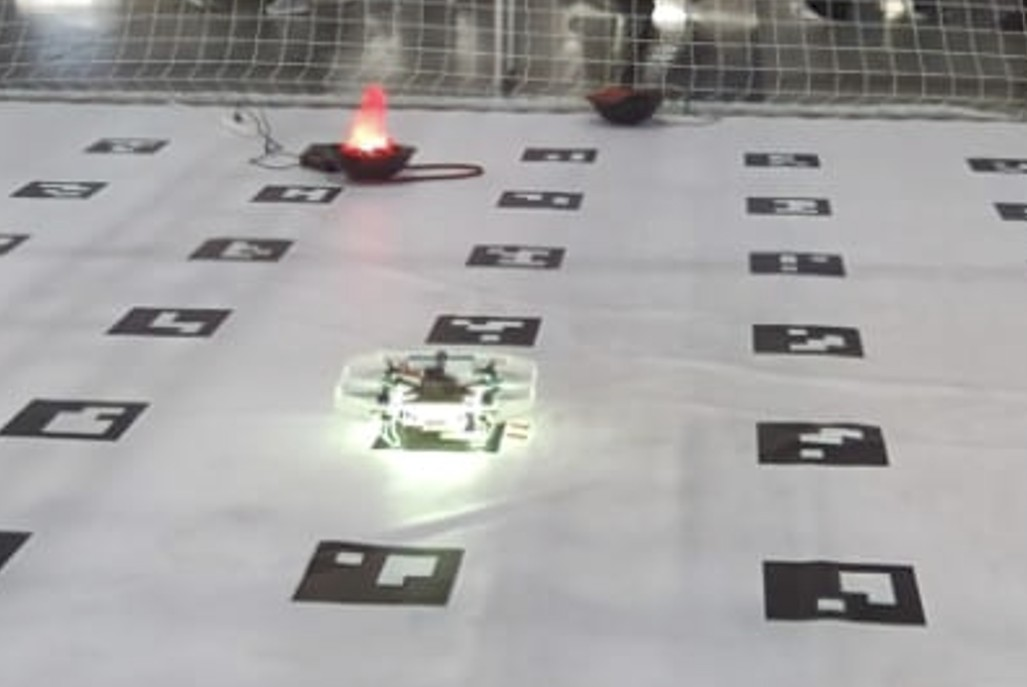
\includegraphics[height=3.3cm]{figures/photo_landing.png}
\caption{Module~B flights, 9--11 Nov 2026: hover test, aircraft surveying the test area, autonomous landing.}
\end{figure}

\begin{figure}[H]
\centering
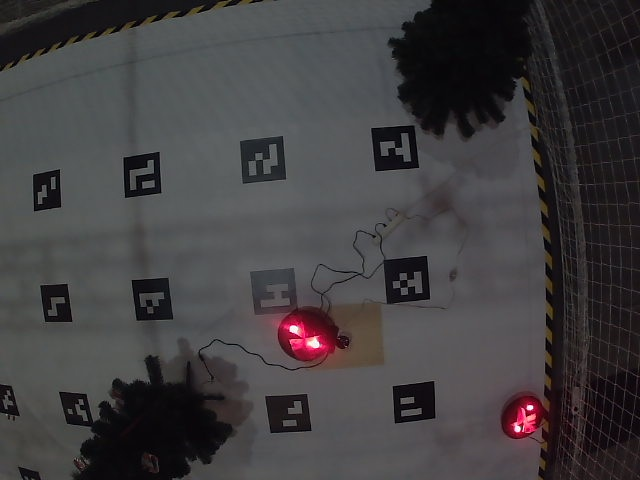
\includegraphics[height=2.6cm]{figures/ev_obj005_fire_rgb_start.jpg}\hfill
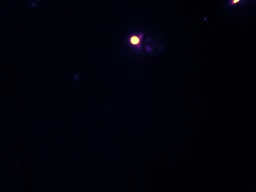
\includegraphics[height=2.6cm]{figures/ev_obj005_fire_thermal_start.jpg}\hfill
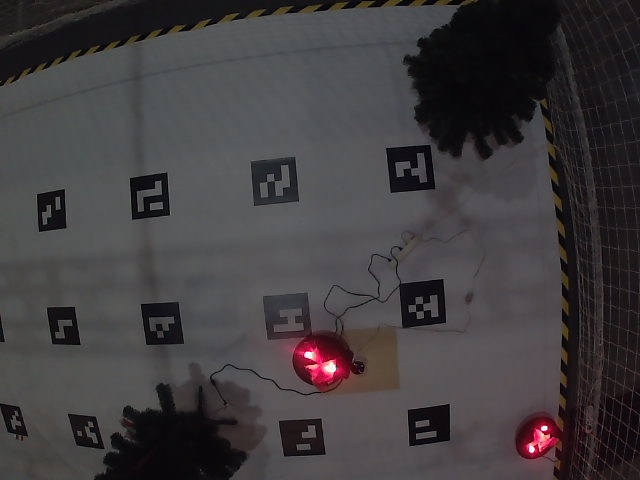
\includegraphics[height=2.6cm]{figures/ev_obj003_tree_rgb.jpg}\hfill
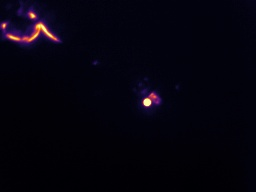
\includegraphics[height=2.6cm]{figures/ev_obj009_tree_fire_thermal_start.jpg}
\caption{Snapshots taken automatically by the drone: campfire (RGB, thermal), tree, tree heat band. This is the output the customer pays for.}
\end{figure}

\begin{table}[H]
\centering\small
\caption{Each economic assumption and the Module~B result behind it}
\label{tab:trace}
\begin{tabularx}{\textwidth}{|L{4.0cm}|L{5.6cm}|Y|}
\hline
\rowcolor{headgray}\head{Assumption} & \head{Module B evidence} & \head{Pilot must confirm} \\ \hline
0.5 FTE runs two UAVs & C1: 15/15 missions, no manual piloting & long field days \\ \hline
UAV can replace patrol checks & C2: mAP@0.5 = 0.993; flame found 15/15 & forest scale \\ \hline
No paid video data link & C4: NPU $\ge$ 10\,FPS in $>$ 90\,\% of flight & --- \\ \hline
Crew sent straight to the point & C5: positions repeat within 0.28\,m & GNSS outdoors \\ \hline
Low accident / insurance cost & C7: return within 0.18\,m; 0 crashes in 61 starts & full season \\ \hline
\end{tabularx}
\end{table}

% ------------------------------------------------------------------ 3
\section{Input Parameters and Assumptions}

\begin{table}[H]
\centering\small
\caption{Model inputs (change any value in \file{econ\_model.py} and every table and chart updates)}
\label{tab:inputs}
\begin{tabularx}{\textwidth}{|L{5.3cm}|L{0.9cm}|R{2.4cm}|Y|}
\hline
\rowcolor{headgray}\head{Parameter} & \head{Symbol} & \head{Value} & \head{Source / status} \\ \hline
Deployment scale & --- & 1 district, 2 UAVs & team model \\ \hline
Assessment horizon & $T$ & 5 years & team model \\ \hline
Discount rate & $r$ & 18\,\% & \src{key rate 14\,\% [7]} + 4\,pp risk \\ \hline
Exchange rates & --- & 82.75 / 92.39 & \src{RUB per USD / EUR, CBR 10 Nov 2026 [8]} \\ \hline
Capital expenditure & $K$ & 3\,500\,000\rub & Table~\ref{tab:cb} \\ \hline
Operating expenditure, year 1 & $O_1$ & 1\,400\,000\rub & Table~\ref{tab:cb} \\ \hline
OPEX escalation & $g$ & 7\,\%/yr & \est{} CBR inflation forecast 6--7\,\% \\ \hline
Benefit ramp-up & $q_t$ & 60\,\%, then 100\,\% & \est{} year 1 = deployment \\ \hline
Residual value, year 5 & $S$ & 300\,000\rub & \est{} resale \\ \hline
\multicolumn{4}{|l|}{\textit{Baseline (current practice), same district and period}} \\ \hline
Patrol flight hours / price per hour & $H$, $p_H$ & 60\,h; 60\,000\rub & \est{} customer records / tenders [10] \\ \hline
Share of patrol hours taken over & $s_H$ & 50\,\% & \est{} \\ \hline
Ground trips / cost per trip & $N_G$, $p_G$ & 100; 8\,000\rub & \est{} 2 people + vehicle \\ \hline
Share of trips replaced & $s_G$ & 50\,\% & \est{} \\ \hline
\multicolumn{4}{|l|}{\textit{Avoided damage}} \\ \hline
Fires caught early / ha saved / RUB per ha & $n_F$, $A$, $d$ & 2; 10\,ha; 150\,000 & \est{} key uncertainty (Section~9) \\ \hline
\end{tabularx}
\end{table}
{\small Excluded: taxes, financing, depreciation. Baseline prices are held flat while our OPEX grows 7\,\%/yr (conservative).}

% ------------------------------------------------------------------ 4
\section{Cost-and-Benefit Calculation Table}

\begin{longtable}{|L{0.7cm}|L{3.1cm}|L{5.0cm}|R{2.5cm}|L{3.3cm}|}
\caption{Cost and benefit items (assignment format)}\label{tab:cb}\\
\hline
\rowcolor{headgray}\head{No.} & \head{Cost / benefit item} & \head{Description} & \head{Amount} & \head{Comments} \\ \hline
\endfirsthead
\hline
\rowcolor{headgray}\head{No.} & \head{Cost / benefit item} & \head{Description} & \head{Amount} & \head{Comments} \\ \hline
\endhead
\multicolumn{5}{|l|}{\textbf{1. Development and capital costs (one-time, year 0)}} \\ \hline
K1 & UAVs with payload & 2 $\times$ PX4 multirotor + Orange Pi 5 Pro + TR256i + RGB + rangefinder & 1\,800\,000\rub & Table~\ref{tab:k1} \\ \hline
K2 & Software development & detection, navigation, tracking, safety, dashboard & 1\,200\,000\rub & paid once \\ \hline
K3 & Ground equipment & laptop, batteries, chargers, cases & 300\,000\rub & \est{} \\ \hline
K4 & Training & 2 operators, certification & 200\,000\rub & \est{} \\ \hline
 & \textbf{Total CAPEX} & & \textbf{3\,500\,000\rub} & \\ \hline
\multicolumn{5}{|l|}{\textbf{2. Operating costs (per year, year 1; +7\,\%/yr)}} \\ \hline
O1 & Operator & 0.5 FTE incl. payroll taxes & 900\,000\rub & autonomy: 1 person, 2 UAVs \\ \hline
O2 & Maintenance & spares, propellers, batteries & 350\,000\rub & \est{} \\ \hline
O3 & Insurance, registration & insurance, registration, mobile data & 150\,000\rub & no video link needed \\ \hline
 & \textbf{Total OPEX} & & \textbf{1\,400\,000\rub/yr} & \\ \hline
\multicolumn{5}{|l|}{\textbf{3. Resource savings and benefits (per full year)}} \\ \hline
S1 & Fewer patrol flights & $H p_H s_H$ = 60 $\times$ 60\,000 $\times$ 50\,\% & 1\,800\,000\rub & cash \\ \hline
S2 & Fewer ground trips & $N_G p_G s_G$ = 100 $\times$ 8\,000 $\times$ 50\,\% & 400\,000\rub & cash \\ \hline
S3 & Avoided fire damage & $n_F A d$ = 2 $\times$ 10\,ha $\times$ 150\,000 & 3\,000\,000\rub & forest owner \\ \hline
 & \textbf{Total benefits} & & \textbf{5\,200\,000\rub/yr} & 60\,\% in year 1 \\ \hline
R1 & Residual value & resale of UAVs and kit, year 5 & 300\,000\rub & \est{} \\ \hline
\end{longtable}

\subsection{Resource bill of one UAV (K1)}
\begin{figure}[H]
\centering
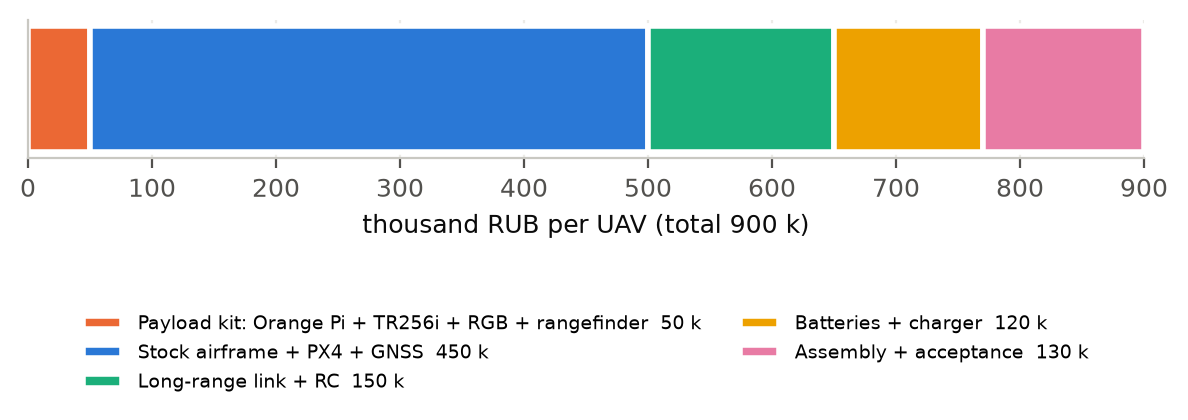
\includegraphics[width=0.92\textwidth]{figures/fig_uav_cost.png}
\caption{The ``smart'' payload is only 50\,000\rub\ (5.6\,\%) of a 900\,000\rub\ UAV; the rest is a standard PX4 drone.}
\end{figure}

\begin{table}[H]
\centering\small
\caption{Bill of major resources for one field UAV (stock components)}
\label{tab:k1}
\begin{tabularx}{\textwidth}{|L{0.5cm}|L{4.6cm}|L{0.6cm}|R{1.7cm}|Y|}
\hline
\rowcolor{headgray}\head{No.} & \head{Resource} & \head{Qty} & \head{RUB} & \head{Price source} \\ \hline
a & Orange Pi 5 Pro 8\,GB (6\,TOPS NPU) & 1 & 17\,957 & \src{USD 216.99, Amazon US [11]} \\ \hline
a & Mileseey TR256i thermal camera 256$\times$192 & 1 & 20\,233 & \src{EUR 218.99, AiO.lv [12]} \\ \hline
b & RGB camera, VL53L1X, cables, mounts & 1 set & 11\,810 & \est{} \\ \hline
c & 10'' multirotor, motors, PX4 FC, GNSS & 1 & 450\,000 & \est{} SKYRIS-class, quote required \\ \hline
d & Long-range telemetry / video link, RC & 1 & 150\,000 & \est{} \\ \hline
e & Six 6S batteries + charger & 1 set & 120\,000 & \est{} \\ \hline
f & Assembly, software install, acceptance flights & 1 & 130\,000 & \est{} Module~B procedure \\ \hline
 & \textbf{Total per UAV} & & \textbf{900\,000} & $\times$ 2 = K1 \\ \hline
\end{tabularx}
\end{table}

% ------------------------------------------------------------------ 5
\section{Calculation Relationships}
\begin{align}
B &= H p_H s_H + N_G p_G s_G + n_F A d, & B_t &= q_t B, & O_t &= O_1 (1+g)^{t-1}\\
CF_0 &= -K, & CF_t &= B_t - O_t + [t=T]\,S, & \mathrm{NPV} &= \textstyle\sum_{t=0}^{T} CF_t/(1+r)^t\\
0 &= \textstyle\sum_{t=0}^{T} CF_t/(1+\mathrm{IRR})^t, & \mathrm{ROI} &= \dfrac{\sum_{t=1}^{T} CF_t - K}{K}, & \text{Payback} &= (t^*-1) + \dfrac{-C_{t^*-1}}{CF_{t^*}}
\end{align}
{\small $C_t$ = cumulative cash flow, $t^*$ = first year with $C_t \ge 0$; if $C_T<0$ the payback is ``not within horizon''.
Same functions as the team's \file{econ.py} and the Excel export (\texttt{NPV()}, \texttt{IRR()}). The script asserts NPV = 6\,205\,125\rub.}

% ------------------------------------------------------------------ 6
\section{Cash Flow and Efficiency Indicators}

\begin{table}[H]
\centering\small
\caption{Base-case cash flow, RUB}
\begin{tabularx}{\textwidth}{|c|R{1.9cm}|R{1.9cm}|R{1.5cm}|R{2.0cm}|R{2.0cm}|R{2.0cm}|Y|}
\hline
\rowcolor{headgray}\head{Year} & \head{Benefits} & \head{OPEX} & \head{Residual} & \head{Net CF} & \head{Cumulative} & \head{Discounted CF} & \head{Cum. disc.} \\ \hline
0 & --- & --- & --- & $-$3\,500\,000 & $-$3\,500\,000 & $-$3\,500\,000 & $-$3\,500\,000 \\ \hline
1 & 3\,120\,000 & 1\,400\,000 & --- & 1\,720\,000 & $-$1\,780\,000 & 1\,457\,627 & $-$2\,042\,373 \\ \hline
2 & 5\,200\,000 & 1\,498\,000 & --- & 3\,702\,000 & 1\,922\,000 & 2\,658\,719 & 616\,346 \\ \hline
3 & 5\,200\,000 & 1\,602\,860 & --- & 3\,597\,140 & 5\,519\,140 & 2\,189\,330 & 2\,805\,676 \\ \hline
4 & 5\,200\,000 & 1\,715\,060 & --- & 3\,484\,940 & 9\,004\,080 & 1\,797\,493 & 4\,603\,170 \\ \hline
5 & 5\,200\,000 & 1\,835\,114 & 300\,000 & 3\,664\,886 & 12\,668\,965 & 1\,601\,955 & \textbf{6\,205\,125} \\ \hline
\end{tabularx}
\end{table}

\begin{table}[H]
\centering\small
\caption{Economic efficiency indicators}
\begin{tabularx}{\textwidth}{|L{4.0cm}|R{2.6cm}|Y|}
\hline
\rowcolor{headgray}\head{Indicator} & \head{Value} & \head{Calculation} \\ \hline
Simple payback & \textbf{1.48 years} & $1 + 1\,780\,000 / 3\,702\,000$ \\ \hline
Discounted payback & \textbf{1.77 years} & $1 + 2\,042\,373 / 2\,658\,719$ \\ \hline
ROI (5 years) & \textbf{362.0\,\%} & $(16\,168\,966 - 3\,500\,000) / 3\,500\,000$ \\ \hline
NPV at 18\,\% & \textbf{6\,205\,125\rub} & $>0$ creates value \\ \hline
IRR & \textbf{74.1\,\%} & $>$ 18\,\% hurdle \\ \hline
Profitability index & 2.77 & $(\mathrm{NPV}+K)/K$ \\ \hline
Break-even benefit level & 57.2\,\% & NPV = 0 if benefits fall 42.8\,\% \\ \hline
\end{tabularx}
\end{table}

\begin{figure}[H]
\centering
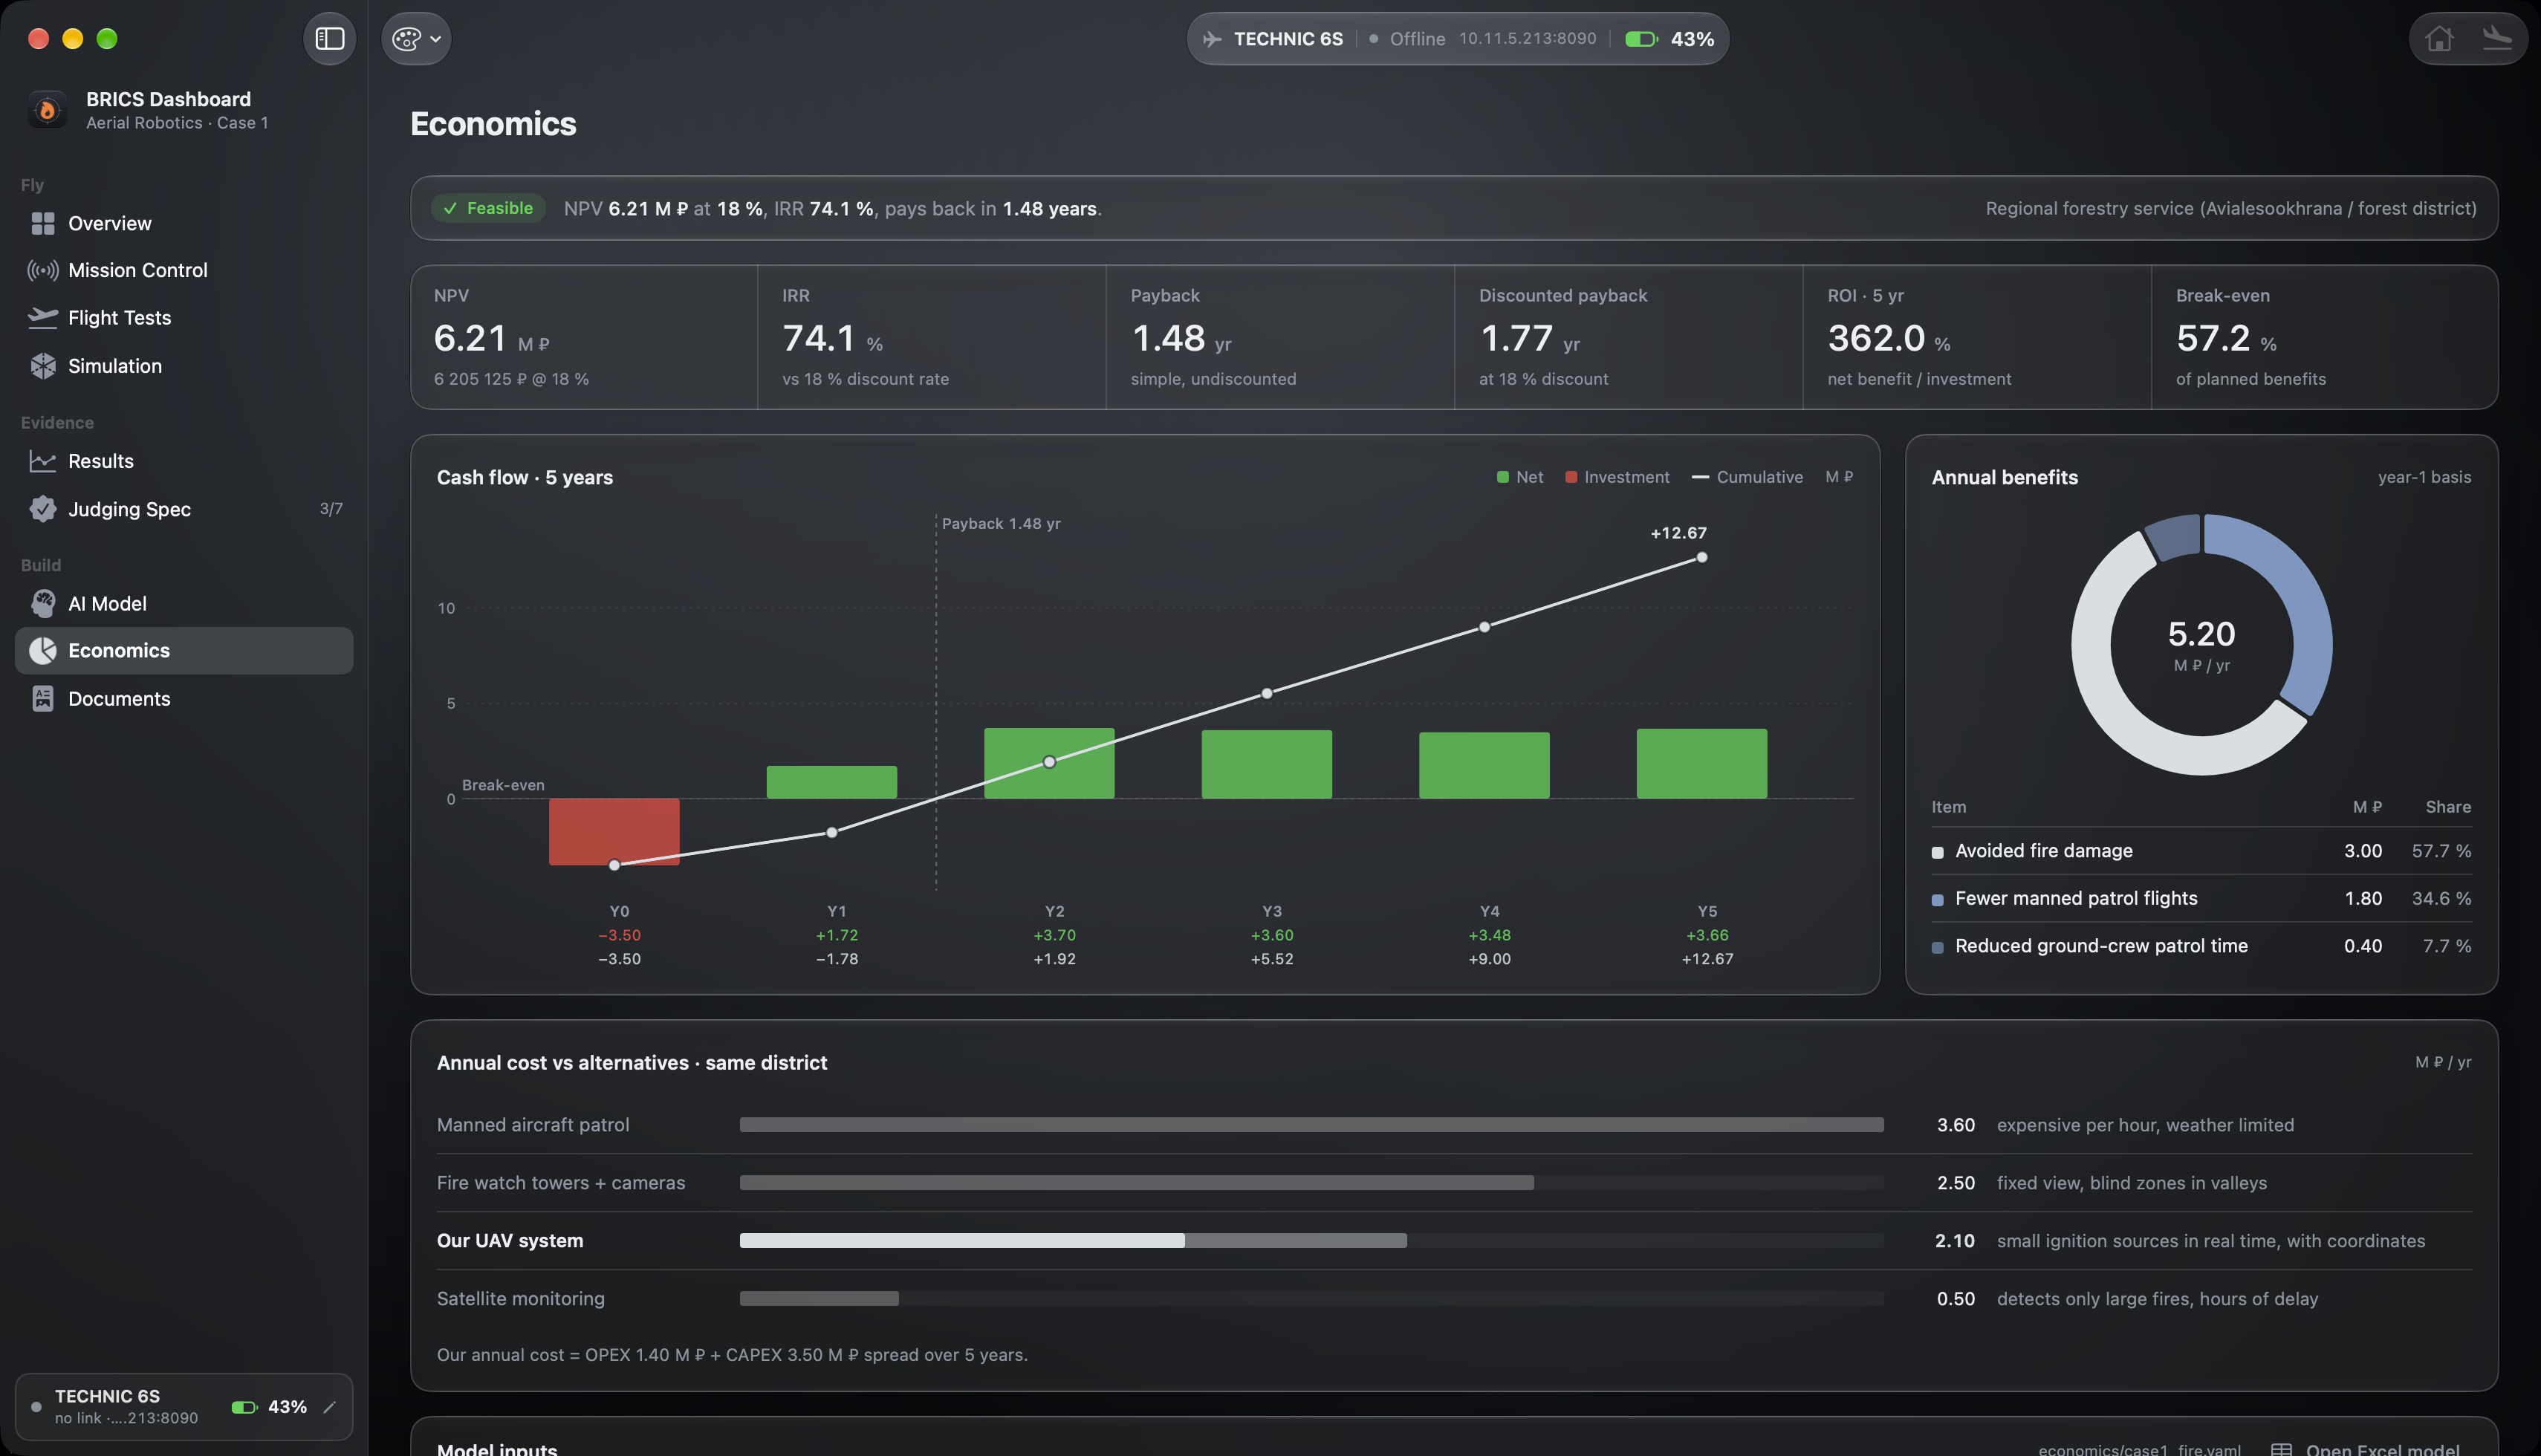
\includegraphics[width=\textwidth]{figures/dash_economics.png}
\caption{Team dashboard, Economics page (12 Nov 2026): same NPV, IRR, payback and ROI, read from the same model file.}
\end{figure}

% ------------------------------------------------------------------ 7
\section{Comparison of Technical Options}
\textbf{Same scope for all options:} one district, 5 years, the baseline's 60 patrol hours and 100 ground trips per year.
Both UAV options take over the same 50\,\% of that work.

\begin{table}[H]
\centering\small
\caption{Three ways to do the same job}
\begin{tabularx}{\textwidth}{|L{2.4cm}|Y|Y|Y|}
\hline
\rowcolor{headgray} & \head{Baseline (today)} & \head{Option A --- this project} & \head{Option B --- COTS drone} \\ \hline
Equipment & light aircraft + ground crew & 2 PX4 drones + Orange Pi + TR256i + our software & 2 $\times$ DJI Mavic 3 Thermal \\ \hline
Finding a fire & observer / crew on site & onboard NN, auto coordinates and log & pilot flies, person watches video \\ \hline
UAV staff & --- & 0.5 FTE & 1.0 FTE \\ \hline
Data link & --- & none (on board) & live video required \\ \hline
Supply risk & low & stock parts, many suppliers & single vendor, uncertain in Russia \\ \hline
\end{tabularx}
\end{table}

\begin{table}[H]
\centering\small
\caption{Bill of major resources --- Option B}
\label{tab:optb}
\begin{tabularx}{\textwidth}{|L{0.6cm}|L{4.6cm}|L{0.8cm}|R{2.2cm}|Y|}
\hline
\rowcolor{headgray}\head{No.} & \head{Resource} & \head{Qty} & \head{RUB} & \head{Price source} \\ \hline
B1 & DJI Mavic 3 Thermal (M3T) & 2 & 1\,126\,939 & \src{USD 6\,809 each [13]} \\ \hline
B2--B5 & batteries/hub; review laptop; manual GIS reporting; training & --- & 900\,000 & \est{} 250 + 150 + 300 + 200\,k \\ \hline
 & \textbf{CAPEX Option B} & & \textbf{2\,026\,939} & \\ \hline
P1--P3 & pilot/analyst 1.0 FTE; DJI Care; insurance & --- & 2\,200\,000/yr & \est{} 1\,800 + 250 + 150\,k \\ \hline
\end{tabularx}
\end{table}

\begin{figure}[H]
\centering
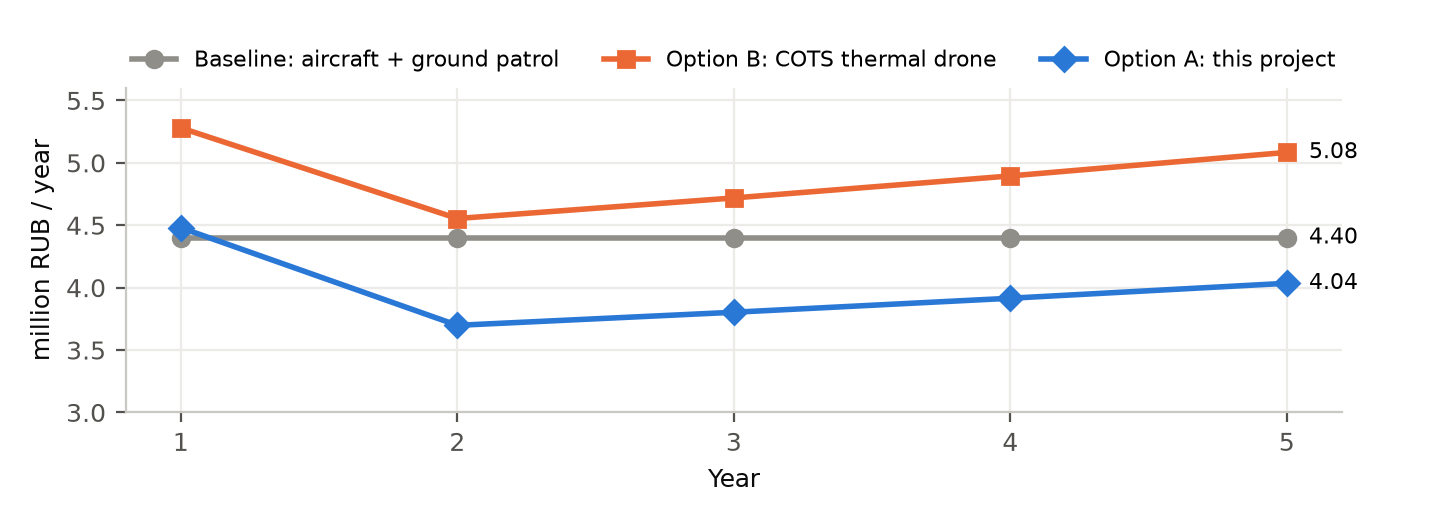
\includegraphics[width=0.92\textwidth]{figures/fig_annual_cost.png}
\caption{Cost per year of the same district service. Option A is the cheapest from year 2; Option B never beats today's practice.}
\end{figure}

\begin{figure}[H]
\centering
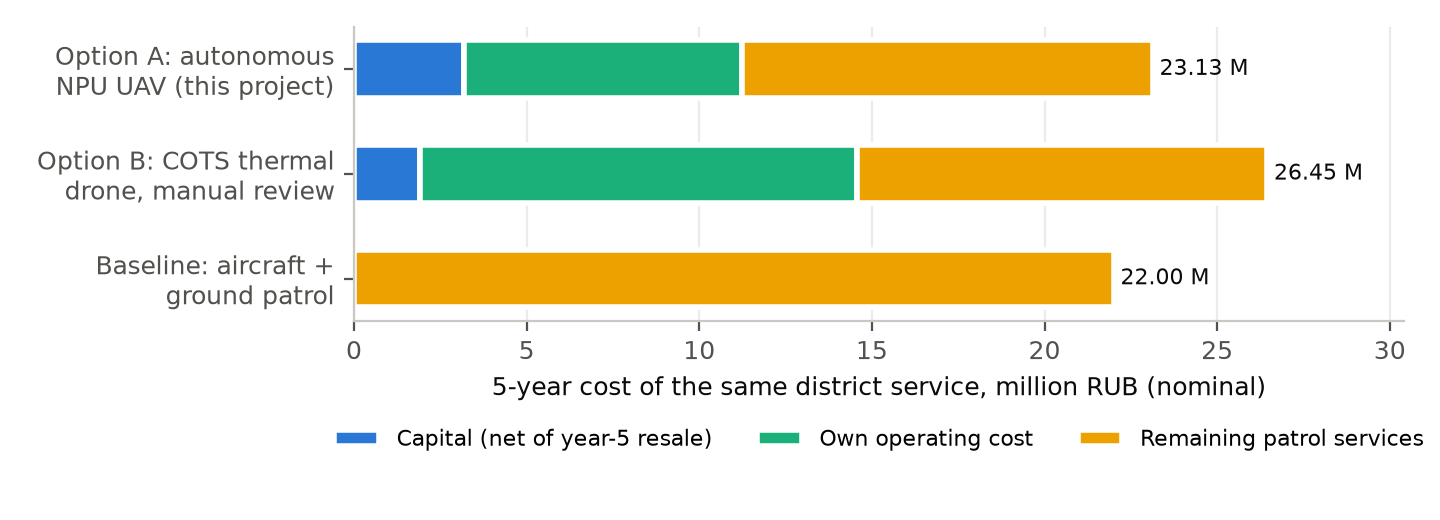
\includegraphics[width=0.92\textwidth]{figures/fig_tco.png}
\caption{Five-year total for the same work.}
\end{figure}

\begin{table}[H]
\centering\small
\caption{Savings (same scope, period and units)}
\begin{tabularx}{\textwidth}{|L{6.6cm}|R{2.6cm}|R{1.5cm}|Y|}
\hline
\rowcolor{headgray}\head{Comparison} & \head{Saving, RUB} & \head{\%} & \head{Result} \\ \hline
A vs B, 5 years nominal & 3\,314\,836 & 12.5\,\% & \textbf{A cheaper} \\ \hline
A vs B, present value at 18\,\% & 1\,422\,860 & 8.2\,\% & \textbf{A cheaper} \\ \hline
A vs baseline, year 2 (steady state) & 702\,000 & 16.0\,\% & A cheaper every year from year 2 \\ \hline
A vs baseline, 5 years, cash only & $-$1\,131\,035 & $-$5.1\,\% & \textbf{not paid back in 5 years} \\ \hline
A vs baseline, PV, cash only (= NPV S-1) & $-$2\,159\,439 & & \\ \hline
A vs baseline, incl. avoided damage (NPV) & 6\,205\,125 & & \textbf{feasible} \\ \hline
\end{tabularx}
\end{table}

\begin{takeaway}
\textbf{Option A is selected:} 1.47\,M\rub\ more CAPEX than Option B, but half the staff time, so 3.31\,M\rub\ (12.5\,\%)
cheaper over 5 years. The innovation is the software: the same stock drone flies and detects without a pilot or a video watcher.
\end{takeaway}

% ------------------------------------------------------------------ 8
\section{Software-Only Deployment and Scaling}

\begin{figure}[H]
\centering
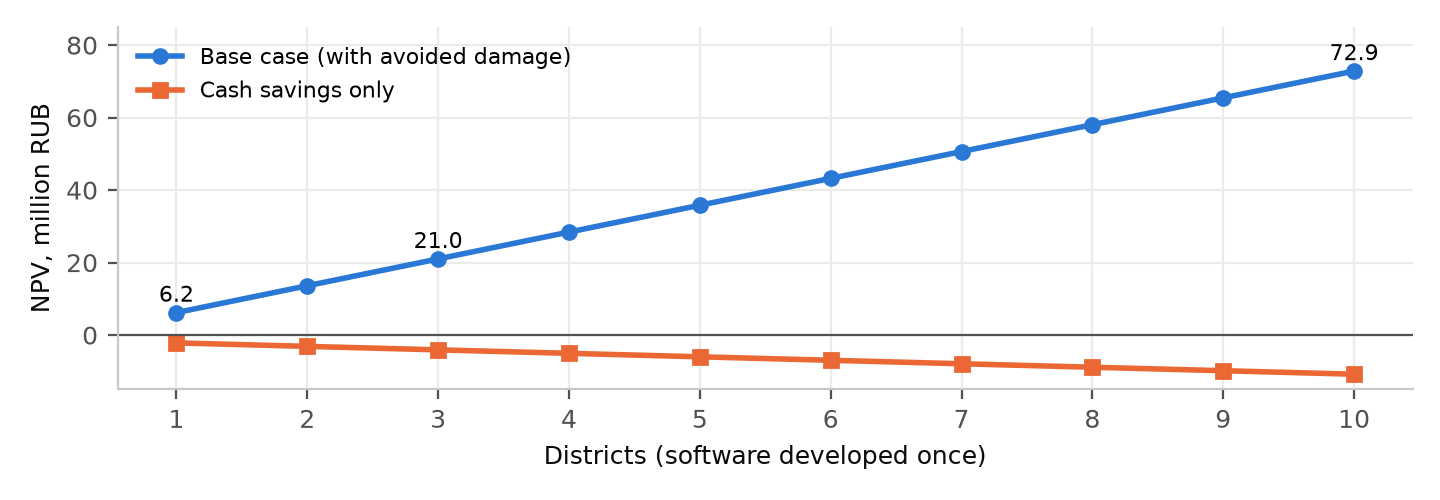
\includegraphics[width=0.92\textwidth]{figures/fig_region.png}
\caption{NPV by number of districts. Software is paid once; each extra district adds 2.3\,M\rub\ CAPEX.}
\end{figure}

\begin{table}[H]
\centering\small
\caption{Deployment variants (5 years, 18\,\%)}
\begin{tabularx}{\textwidth}{|L{4.6cm}|R{1.9cm}|R{2.1cm}|R{1.3cm}|R{1.4cm}|Y|}
\hline
\rowcolor{headgray}\head{Variant} & \head{CAPEX} & \head{NPV} & \head{IRR} & \head{Payback} & \head{Cash only} \\ \hline
Base: 1 district, new UAVs & 3\,500\,000 & 6\,205\,125 & 74.1\,\% & 1.48 yr & no payback \\ \hline
\textbf{Retrofit: customer's own drones} & 2\,060\,000 & 7\,645\,125 & 122.3\,\% & 1.09 yr & \textbf{payback 4.54 yr} \\ \hline
Region: 3 districts & 8\,100\,000 & 21\,015\,374 & 95.4\,\% & 1.26 yr & no payback \\ \hline
Region: 10 districts & 24\,200\,000 & 72\,851\,248 & 105.6\,\% & 1.19 yr & no payback \\ \hline
\end{tabularx}
\end{table}
{\small Retrofit CAPEX $= 2 \times (50\,000 + 130\,000) + 1\,200\,000 + 300\,000 + 200\,000 = 2\,060\,000$\rub\ (payload kit,
installation, software, ground kit, training).}

\begin{takeaway}
\textbf{Fastest route to market:} sell the software + payload kit to services that already fly PX4 drones. No new aircraft,
and cash payback within the horizon (4.54 years) even without counting avoided damage.
\end{takeaway}

% ------------------------------------------------------------------ 9
\section{Risk and Sensitivity Analysis}

\begin{figure}[H]
\centering
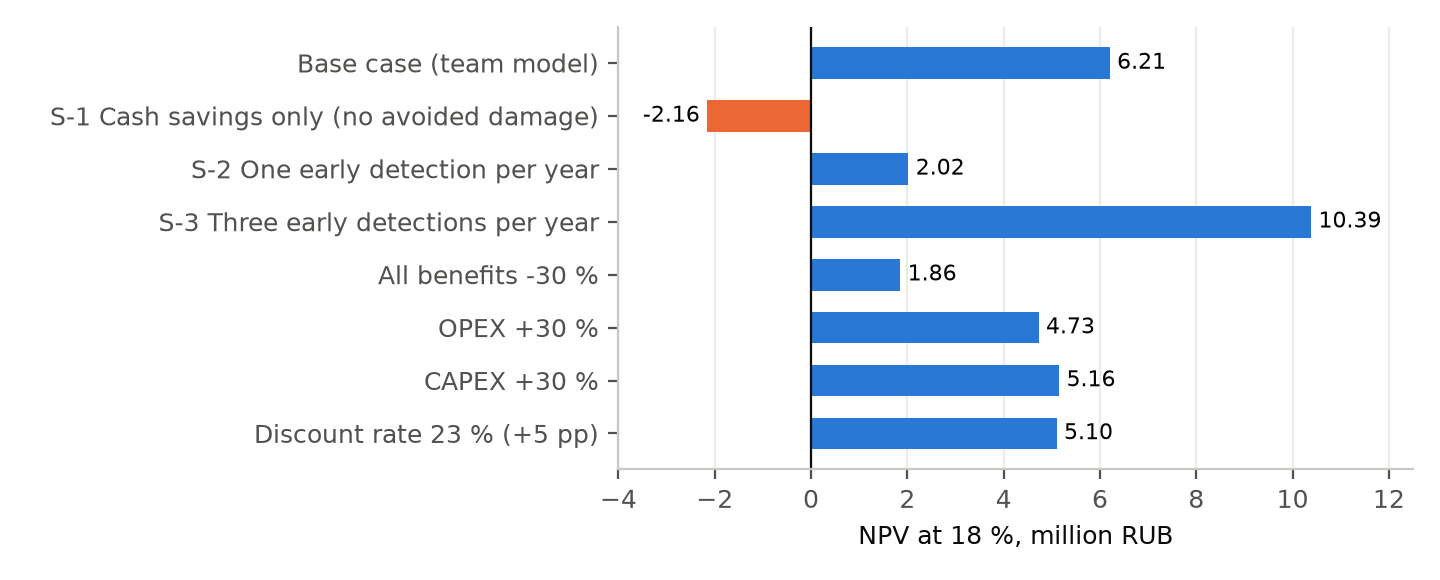
\includegraphics[width=0.92\textwidth]{figures/fig_scenarios.png}
\caption{NPV under the justified scenarios and one-factor changes.}
\end{figure}

\begin{table}[H]
\centering\small
\caption{Scenario indicators}
\begin{tabularx}{\textwidth}{|Y|R{2.2cm}|R{1.5cm}|R{2.0cm}|R{2.0cm}|}
\hline
\rowcolor{headgray}\head{Scenario} & \head{NPV, RUB} & \head{IRR} & \head{Payback} & \head{Disc. payback} \\ \hline
Base case & 6\,205\,125 & 74.1\,\% & 1.48 yr & 1.77 yr \\ \hline
S-1 Cash savings only & $-$2\,159\,439 & $-$10.3\,\% & not within 5 yr & not within 5 yr \\ \hline
S-2 One early detection / yr & 2\,022\,843 & 38.4\,\% & 2.23 yr & 2.96 yr \\ \hline
S-3 Three early detections / yr & 10\,387\,407 & 105.9\,\% & 1.17 yr & 1.34 yr \\ \hline
All benefits $-30\,\%$ & 1\,855\,552 & 36.8\,\% & 2.28 yr & 3.06 yr \\ \hline
OPEX $+30\,\%$ & 4\,727\,749 & 61.7\,\% & 1.68 yr & 2.03 yr \\ \hline
CAPEX $+30\,\%$ & 5\,155\,125 & 56.1\,\% & 1.76 yr & 2.20 yr \\ \hline
Discount rate 23\,\% & 5\,102\,709 & 74.1\,\% & 1.48 yr & 1.86 yr \\ \hline
\end{tabularx}
\end{table}

\begin{figure}[H]
\centering
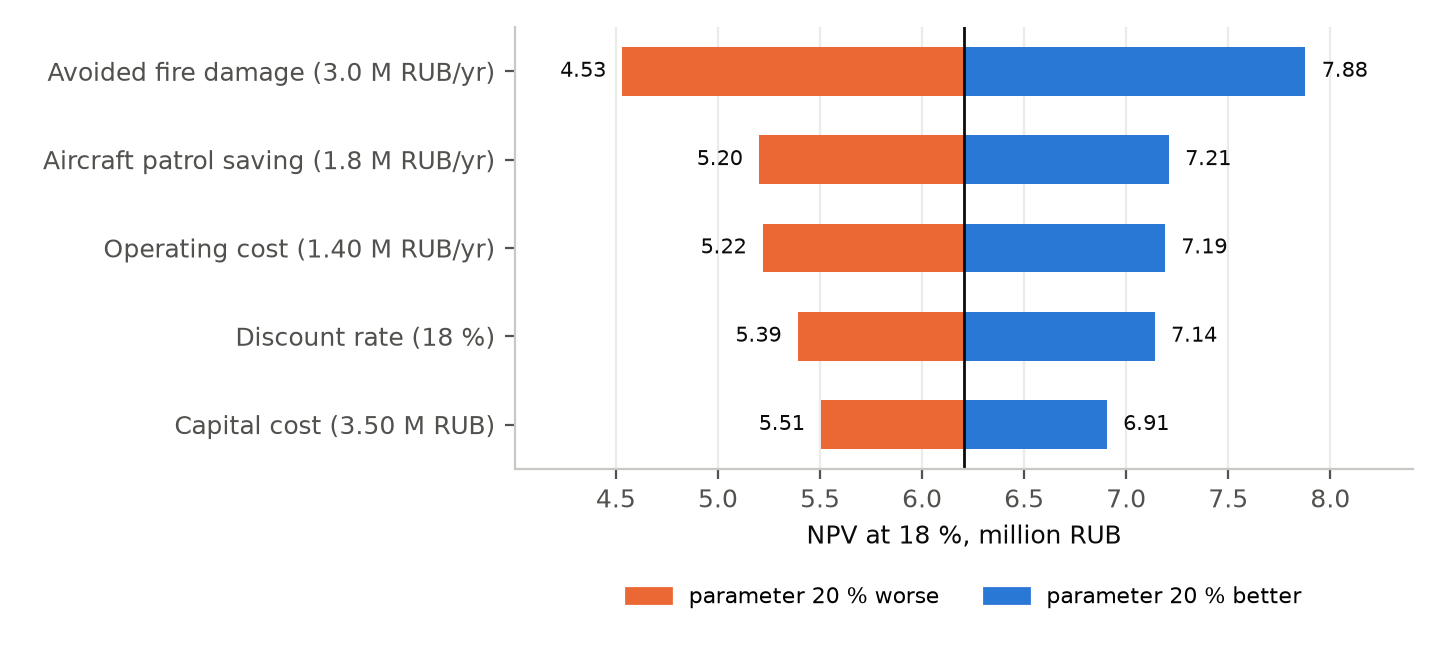
\includegraphics[width=0.92\textwidth]{figures/fig_tornado.png}
\caption{NPV with each parameter $\pm$20\,\%. Avoided damage matters most; capital cost matters least.}
\end{figure}

\begin{figure}[H]
\centering
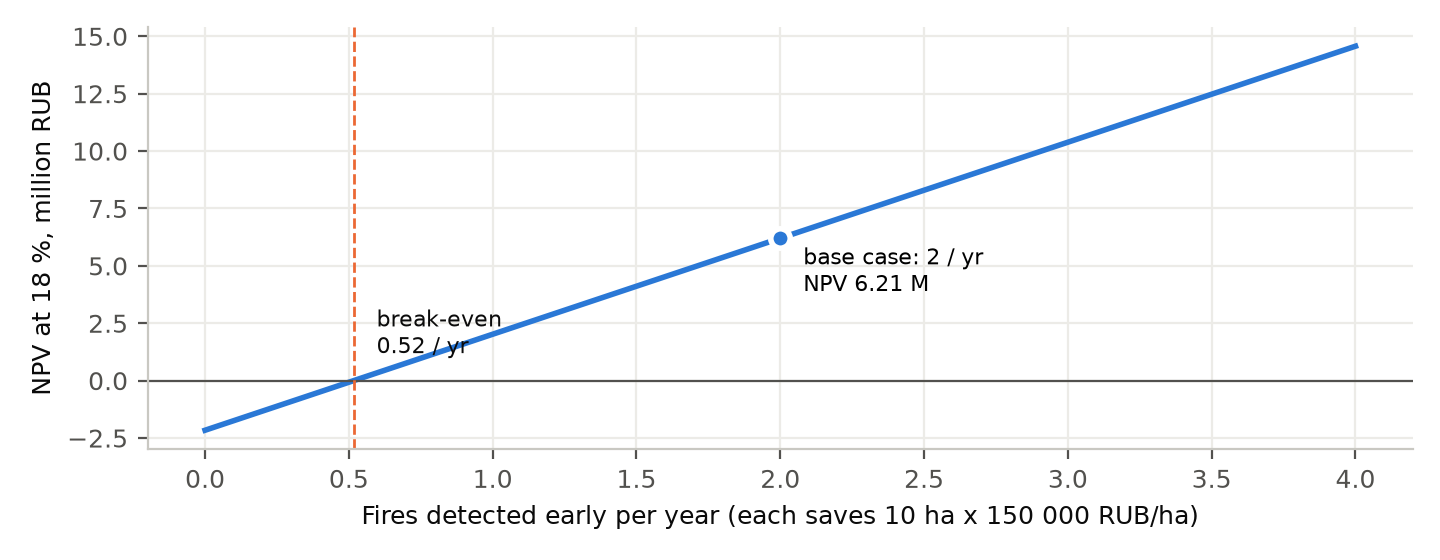
\includegraphics[width=0.92\textwidth]{figures/fig_breakeven.png}
\caption{Key parameter: NPV vs fires caught early per year. Break-even 0.52 --- one prevented 10\,ha fire every two years.}
\label{fig:be}
\end{figure}

\begin{caution}
\textbf{Cash-only break-even:} without avoided damage, the project needs a district with at least \textbf{85.8 patrol hours/yr}
(baseline 60). Bigger districts are feasible on cash savings alone.
\end{caution}

\begin{table}[H]
\centering\small
\caption{Principal risks}
\begin{tabularx}{\textwidth}{|L{4.0cm}|L{4.0cm}|Y|}
\hline
\rowcolor{headgray}\head{Risk} & \head{Effect} & \head{Mitigation} \\ \hline
Fewer fires caught early & NPV $<0$ below 0.52/yr & measure in the pilot season \\ \hline
Patrol hours not actually cut & S1 not cash & agree replaced flights with customer \\ \hline
Arena $\ne$ forest & lower benefits & outdoor GNSS test before pilot \\ \hline
Hardware prices rise & CAPEX $+30\,\%$: NPV still 5.16\,M & stock parts; retrofit variant \\ \hline
\end{tabularx}
\end{table}

% ------------------------------------------------------------------ 10
\section{Social and Environmental Effects}
{\small Not included in NPV or ROI.}

\begin{center}
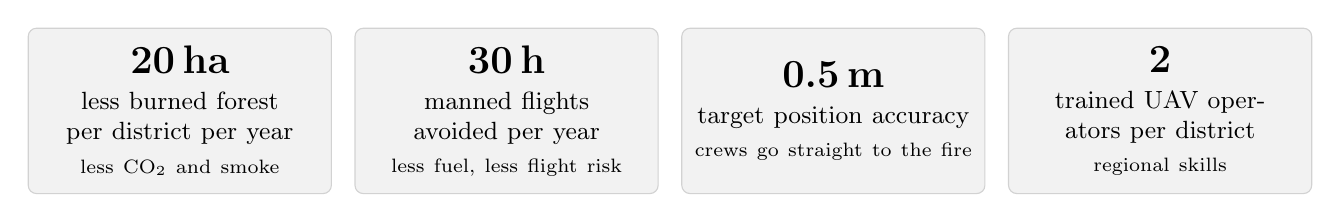
\begin{tikzpicture}[tile/.style={draw=gray!35,fill=headgray,rounded corners=3pt,minimum width=3.85cm,minimum height=2.1cm,align=center,text width=3.6cm}]
\node[tile] (a) at (0,0) {{\Large\bfseries 20\,ha}\\[2pt]\small less burned forest per district per year\\\scriptsize less CO$_2$ and smoke};
\node[tile] (b) at (4.15,0) {{\Large\bfseries 30\,h}\\[2pt]\small manned flights avoided per year\\\scriptsize less fuel, less flight risk};
\node[tile] (c) at (8.3,0) {{\Large\bfseries 0.5\,m}\\[2pt]\small target position accuracy\\\scriptsize crews go straight to the fire};
\node[tile] (d) at (12.45,0) {{\Large\bfseries 2}\\[2pt]\small trained UAV operators per district\\\scriptsize regional skills};
\end{tikzpicture}
\end{center}

% ------------------------------------------------------------------ 11
\section{Conclusions and Recommendations}

\begin{takeaway}
\textbf{Economically feasible.} NPV 6.21\,M\rub, IRR 74.1\,\%, ROI 362\,\%, payback 1.48 years; 12.5\,\% cheaper than the commercial
alternative. Condition: at least 0.52 fires per year caught early, or a district with at least 86 patrol hours per year.
\end{takeaway}

\begin{tabularx}{\textwidth}{@{}Y Y@{}}
\textbf{Key factors} & \textbf{Proposals to cut cost / raise benefit} \\
\begin{enumerate}[leftmargin=1.4em]
\item Fires caught early and area saved
\item Patrol hours actually replaced
\item Staff time per UAV (autonomy)
\item UAV availability: weather, batteries
\end{enumerate}
&
\begin{itemize}[leftmargin=1.2em]
\item Sell software + kit for drones the customer owns
\item Share the fleet with emergency services
\item Scale to the region: software paid once
\item Plan sorties from satellite alerts (FIRMS)
\end{itemize} \\
\end{tabularx}

\needspace{5cm}
\subsection{Deployment roadmap}
\begin{center}
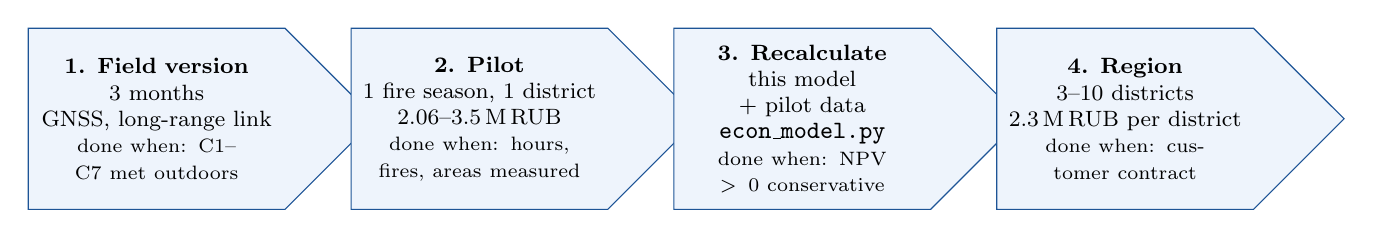
\begin{tikzpicture}[st/.style={signal,signal to=east,draw=vizblue!70!black,fill=vizblue!8,minimum height=2.3cm,
  text width=3.05cm,align=center,font=\footnotesize,inner sep=3pt}]
\node[st] (s1) at (0,0) {\textbf{1. Field version}\\3 months\\GNSS, long-range link\\\scriptsize done when: C1--C7 met outdoors};
\node[st] (s2) at (4.1,0) {\textbf{2. Pilot}\\1 fire season, 1 district\\2.06--3.5\,M\rub\\\scriptsize done when: hours, fires, areas measured};
\node[st] (s3) at (8.2,0) {\textbf{3. Recalculate}\\this model + pilot data\\\file{econ\_model.py}\\\scriptsize done when: NPV $>0$ conservative};
\node[st] (s4) at (12.3,0) {\textbf{4. Region}\\3--10 districts\\2.3\,M\rub\ per district\\\scriptsize done when: customer contract};
\end{tikzpicture}
\end{center}

% ------------------------------------------------------------------ 12
\section{Compliance with Module C Requirements}
\begin{tabularx}{\textwidth}{|Y|L{4.8cm}|L{1.7cm}|}
\hline
\rowcolor{headgray}\head{Requirement (assignment / assessment criteria)} & \head{Where} & \head{Status} \\ \hline
Economic model: rationale, cost categories, benefits & Section 1 & \PASS \\ \hline
Cost-and-benefit calculation table & Table~\ref{tab:cb} & \PASS \\ \hline
Payback, ROI, NPV, IRR & Section 6 & \PASS \\ \hline
Inputs: scale, horizon, CAPEX, OPEX, baseline, formulas, assumptions & Sections 3, 5 & \PASS \\ \hline
Two technical options, resource bills with quantities, prices, sources & Tables~\ref{tab:k1}, \ref{tab:optb} & \PASS \\ \hline
Savings vs baseline, same scope; payback not reached stated explicitly & Section 7 & \PASS \\ \hline
Reproducible: formulas, units, sources, script & Sections 3, 5; \file{econ\_model.py} & \PASS \\ \hline
Scenarios and sensitivity of a key parameter & Section 9 & \PASS \\ \hline
Social and environmental effects & Section 10 & \PASS \\ \hline
Conclusions, key factors, proposals & Section 11 & \PASS \\ \hline
\end{tabularx}

% ------------------------------------------------------------------ references
\section*{References}
\begin{enumerate}[label={[\arabic*]},leftmargin=2.2em,itemsep=0pt]\small
\item HiTech 2026. \textit{Competition Assignment: Aerial Robotics}, Module C.
\item HiTech 2026. \textit{Flying Robotics Competition Tasks}, Case 1 University 2035.
\item HiTech 2026. \textit{Flying Robotics Global Assessment Criteria}, sub-criterion C1.
\item Team ENTITY. \textit{Module A --- Engineering Design and Development}, November 2026.
\item Team ENTITY. \textit{Module B --- Prototype Functional Verification}, 9--11 November 2026.
\item Project repository: \url{https://github.com/kkjjkamal123/BRICS-HiTech-2026-Flying-Robotics}
\item Bank of Russia, key rate decisions 2026. \url{https://cbr.ru/press/keypr/}
\item CBR official exchange rates, 10 Nov 2026. \url{https://investfuture.ru/articles/obzor-valyut-2026-11-10}
\item EMERCOM of Russia \url{https://mchs.gov.ru/}; Rosleskhoz \url{https://rosleshoz.gov.ru/}
\item Unified procurement system (aviation forest-protection tenders). \url{https://zakupki.gov.ru/}
\item Orange Pi 5 Pro 8\,GB price history. \url{https://pricehistory.app/p/orange-pi-5-pro-8gb-rk3588s-lpddr5-Sa85rAce}
\item Mileseey TR256i, AiO.lv. \url{https://aio.lv/en/product--mileseey-tr256ian--12423636.md}
\item DJI Mavic 3T price guide 2026. \url{https://globaldronehq.com/blogs/news/dji-mavic-3-thermal-m3t-specs-price-complete-guide-2026}
\item NASA FIRMS. \url{https://firms.modaps.eosdis.nasa.gov/}
\end{enumerate}

\vspace{6pt}
\begin{center}
\textbf{END OF REPORT --- Module C: Economic Feasibility Assessment}
\end{center}

\end{document}
